\documentclass[10pt, hyperref={unicode}]{beamer}
\usepackage[utf8]{inputenc}
\usepackage{xcolor}
\usepackage{times}
\usetheme{Berlin}
\usepackage[czech]{babel}
\usepackage{listings}
\lstset{language=Pascal, numbers=left, basicstyle=\footnotesize, morekeywords={is, each}}

\title[Dijkstrův grafový algoritmus]{Typografie a publikování -- 5. projekt}
\subtitle{Dijkstrův grafový algoritmus}
\author[Vojtěch Fiala]{Vojtěch Fiala \texorpdfstring{\\ \href{mailto:xfiala61@stud.fit.vutbr.cz}{xfiala61@stud.fit.vutbr.cz}}{}}
\date{\today}
\institute[VUT FIT]{
Vysoké učení technické v Brně\\
Fakulta informačních technologií
}

\begin{document}
    \maketitle

    \begin{frame}{Obsah}
        \tableofcontents
    \end{frame}

    \section{Představení algoritmu}
    \begin{frame}{Představení algoritmu}
    \begin{itemize}
            \item<1-> Byl vytvořen nizozemským informatikem \textbf{Edsgerem Dijkstrou}
            \item<2-> Slouží k nalezení \textbf{nejkratší} cesty v~grafu. 
            \item<3-> Je \textbf{konečný} -- má vždy určitý počet iterací.
            \item<4-> Používá se pouze nad hranově \textbf{kladně} ohodnocenými grafy.
        
			\begin{figure}
            \item<5->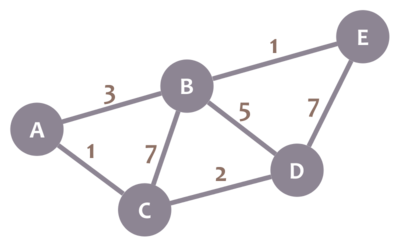
\includegraphics[scale=0.175]{graph.png}
			\caption{\footnotesize{Ukázka kladně ohodnoceného grafu}}
			\end{figure}
			
        \end{itemize}
    \end{frame}
    
    \section{Fungování algoritmu}
    \begin{frame}{Fungování algoritmu}
        \begin{itemize}
            \item<1-> Uzly jsou uchovávány v \textbf{prioritní frontě}, kde jsou seřazeny podle \textbf{vzdálenosti od počátku}.
            \item<2-> V první iteraci počítá pouze s počátkem, který má vzdálenost \textbf{0}, příčemž všechny ostatní uzly mají vzdálenost \textbf{nekonečno}.
            \item<3-> V každém dalším kroku vybere z fronty uzel s nejvyšší prioritou (tzn. uzel s \textbf{nejnižší vzdáleností} od již zpracované části) a~zařadí jej mezi zpracované uzly. 
            \end{itemize}
    \end{frame}
    \begin{frame}{Fungování algoritmu}
        \begin{itemize}
            \item<1-> Dále projde všechny uzly z původního, právě zpracovaného uzlu \textbf{vycházející} a přidá je do fronty, nejsou-li tam již obsaženy.
            \item<2-> Vypočítá, zda-li nejsou blíže počátku, než byly před zařazením právě vybraného uzlu mezi zpracované.
            \item<3-> Algorimus končí v okamžiku, kdy jsou zpracovány všechny uzly -- prioritní fronta je \textbf{prázdná}.
        \end{itemize}
    \end{frame}
    
    \section{Složitost}
    \begin{frame}[fragile]{Složitost}
        \begin{itemize}
            \item<1-> Algoritmus lze naimplementovat s asymptotickou \textbf{složitostí} $O (E + V\log V)$
            \item<2-> $V$ představuje počet uzlů a $E$ počet hran.
        \end{itemize}
    \end{frame}
    
    \section{Pseudokód -- fungování algoritmu}
    \begin{frame}[fragile]{Pseudokód -- fungování algoritmu}
    \begin{lstlisting}[mathescape=true]
function Dijkstra($E$, $V$, $s$):
    for each vertex $v$ in $V$:
        d[$v$] := infinity  
        p[$v$] := undefined
    d[$s$] := 0
    $N$ := $V$
    while $N$ is not empty:
        $u$ := extract_min($N$)                       
        for each neighbor $v$ of $u$:
            alt = d[$u$] + length($u$, $v$)
            if alt < d[$v$]              
                d[$v$] := alt
                p[$v$] := u
    \end{lstlisting}
    \end{frame}

    \section{Zdroje}
    \begin{frame}{Zdroje}
        \begin{thebibliography}{3}
		\bibitem{} Představení algoritmu, pseudokód\\
		\texttt{\footnotesize{\url{https://cs.wikipedia.org/wiki/Dijkstr\%C5\%AFv\_algoritmus}}}

		\bibitem{} Fungování\\
		\texttt{\footnotesize{\url{https://www.algoritmy.net/article/5108/Dijkstruv-algoritmus}}}
		
		\bibitem{} Složitost\\
		\texttt{\footnotesize{\url{http://voho.eu/wiki/algoritmus-dijkstra/}}}
	\end{thebibliography}
    \end{frame}
    
\end{document}
